\documentclass[10pt,a4paper]{scrbook}

% Input Type and AMS-Packages 
\usepackage{amsmath,amsfonts,amssymb,amsthm}
\usepackage{unicode-math}

% Typography
\usepackage{fontspec}
\setmainfont{EB Garamond}
\newfontfamily\headingfont[RawFeature={+c2sc,+scmp},
                           Letters=SmallCaps]{EB Garamond}
\setsansfont[Scale=MatchLowercase]{Open Sans}
\setmonofont[Scale=MatchUppercase]{Fira Mono}
\setmathtt[Scale=MatchUppercase]{Fira Mono}

\renewcommand{\scshape}{\headingfont}

\usepackage{polyglossia}
\setdefaultlanguage[variant=british]{english}
\setotherlanguage{german}
\usepackage{floatrow}
\usepackage{booktabs}

\usepackage{csquotes}
\usepackage{microtype}
\usepackage{enumitem}
\usepackage{subcaption}

\usepackage{letltxmacro}

\newlist{thmlist}{enumerate}{1}			% thmlist-s may only be used in theorem environments
\setlist[thmlist]{label=(\roman{thmlisti}), ref=\thethm.(\roman{thmlisti}),noitemsep}
\newlist{exlist}{enumerate}{1}
\setlist[exlist]{label=(\arabic{exlisti}), ref=(\arabic{exlisti}),noitemsep,leftmargin=0pt,itemindent=2\parindent}
\newlist{plist}{enumerate}{1}
\setlist[plist]{label=(\roman{plisti}), ref=(\roman{plisti}),noitemsep,leftmargin=0pt,itemindent=2\parindent}
\newlist{clist}{enumerate}{2}
\setlist[clist]{label*=(\alph*), ref=(\alph*),noitemsep,leftmargin=0pt,itemindent=2\parindent}

\usepackage{setspace}
\renewcommand{\arraystretch}{1.5}

\usepackage[symbol]{footmisc}		% Use symbols for footnotes
\usepackage{perpage}				% Package to reset counters at the end of each page.
\MakePerPage{footnote}				% Reset footnote-counter at the end of each page

\usepackage{listingsutf8}	% Typeset code.
\lstset{extendedchars=true,
        basicstyle=\ttfamily,
        commentstyle=\color{gray},
        stringstyle=\color{darkgray},
        xleftmargin=\parindent,
        language=haskell}

% BibLaTex
\usepackage[style=numeric,backend=biber]{biblatex}
\addbibresource{./references.bib}


% Math, Operators and Theorems
\usepackage{thmtools}	% More Flexibility in Theorem Styles + Provides in Combination with ref-Packages the 
						% Possibility to Refer to Theorem Style in Reference.
\usepackage{faktor}		% Displays factor groups

\numberwithin{equation}{section}

\DeclareMathOperator{\N}{\mathbb{N}}
\DeclareMathOperator{\Z}{\mathbb{Z}}
\DeclareMathOperator{\Q}{\mathbb{Q}}
\DeclareMathOperator{\R}{\mathbb{R}}
\DeclareMathOperator{\C}{\mathbb{C}}
\DeclareMathOperator{\F}{\mathbb{F}}

\DeclareMathOperator{\Aut}{Aut}
\DeclareMathOperator{\id}{id}

\DeclareMathOperator{\kernel}{ker}
\DeclareMathOperator{\im}{im}
\DeclareMathOperator{\End}{\mathrm{End}}
\DeclareMathOperator{\Hom}{\mathrm{Hom}}
\DeclareMathOperator{\Mod}{\mathrm{mod}}
\DeclareMathOperator{\D}{\mathrm{D}}
\DeclareMathOperator{\lcm}{\mathrm{lcm}}
\DeclareMathOperator{\ord}{\mathrm{ord}}

\newcommand{\sta}{\texttt{§}}
\newcommand{\emp}{\texttt{\_}}
\newcommand{\zer}{\mathtt 0}
\newcommand{\one}{\mathtt 1} 
\newcommand{\sstart}{s_{\text{start}}}
\newcommand{\shalt}{s_{\text{halt}}}
\newcommand{\scheck}{s_{\text{check}}}
\newcommand{\enc}[1]{\ulcorner #1 \urcorner}


\declaretheoremstyle[
    spaceabove=6pt, spacebelow=6pt,
    headfont=\headingfont,
    notefont=\mdseries, notebraces={(}{)},
    bodyfont=\itshape,
    postheadspace=1em
    ]{mythm}
\declaretheoremstyle[
    spaceabove=6pt, spacebelow=6pt,
    headfont=\headingfont,
    notefont=\mdseries, notebraces={(}{)},
    bodyfont=\normalfont,
    postheadspace=1em
    ]{mydef}

\declaretheorem[
	name=Theorem,
    style=mythm,
  	refname={theorem,theorems},		%Lower Case Versions of Theorem Type
  	Refname={Theorem,Theorems},
  	numberwithin=section]{thm}
\declaretheorem[
	name=Lemma,
    style=mythm,
	refname={lemma,lemmas},
	Refname={Lemma,Lemmas},
	sibling=thm]{lem}
\declaretheorem[
	name=Proposition,
    style=mythm,
	refname={proposition,propositions},
	Refname={Proposition,Propositions},
	sibling=thm]{pro}
\declaretheorem[
	name=Corollary,
    style=mythm,
	refname={corollary,corollarys},
	Refname={Corollary,Corollarys},
	sibling=thm]{cor}

\declaretheorem[
	name=Definition,
	style=mydef,
	numbered=no]{defin}
\declaretheorem[
	name=Example,
	style=mydef,
	numbered=no]{exam}
	
\declaretheorem[
	name=remark,
	style=remark,
	numbered=no]{rem}
\renewcommand*{\proofname}{proof}



%\newtheorem{theo}{Theorem}[section]
%\newtheorem{lemma}[theo]{Lemma}
%\newtheorem{prop}[theo]{Proposition}
%\newtheorem{cor}[theo]{Corollary}
%\theoremstyle{definition}
%\newtheorem*{defin}{Definition}
%\newtheorem*{exam}{Example}
%\theoremstyle{remark}
%\newtheorem*{rem}{Remark}

%TikZ and TikZ-Styles
\usepackage{tikz}

\usepackage{pgfcore}
\usetikzlibrary{arrows}

\tikzstyle{every node}=[circle,draw=black,font=\small,text=black,inner sep=1pt, minimum size=5mm]
\tikzstyle{edge from parent}=[draw=black]
\tikzstyle{st}=[black!20, line join=round, line width=2mm]
\tikzstyle{st1}=[black!40, line join=round, line width=2mm]

\tikzstyle{bgn}=[node distance=6mm, font=normal]
\tikzstyle{hlarrow}=[<->, shorten <=1pt, shorten >=1pt, draw, thick]

\tikzstyle{level 1}=[sibling distance=60mm]
\tikzstyle{level 2}=[sibling distance=30mm]
\tikzstyle{level 3}=[sibling distance=15mm]
\tikzstyle{level 4}=[sibling distance=7.5mm]
\tikzstyle{level 5}=[sibling distance=3.75mm, level distance=5mm]


% New- and Renewcommands

\newcommand{\seq}[2][n]{#2_{1},\ldots,#2_{#1}}
\newcommand{\nicefrac}[2]{#1/#2}




% ----------------------------------------------------------
% Only for drafts!
\usepackage{todonotes}
\usepackage{showlabels}	%Used in Drafts to Print references.
%-----------------------------------------------------------



% References
\usepackage{hyperref}
\usepackage[capitalize]{cleveref}

\hypersetup{
	pdftitle={Unbounded Burnside Problem for Groups},
	pdfauthor={Tim Benedikt Herbstrith}}

%\Crefname{thm}{Theorem}{Theorems}
%\Crefname{lem}{Lemma}{Lemmas}
%\Crefname{pro}{Proposition}{Propositions}
%\Crefname{cor}{Corollary}{Corollaries}

%\crefname{thm}{thm.}{thms.}
%\crefname{lem}{lemma}{lemmas.}
%\crefname{pro}{prop.}{props.}
%\crefname{cor}{cor.}{cors.}

\Crefname{thm}{Thm.}{Thms.}
\Crefname{lem}{Lemma}{Lemmas.}
\Crefname{pro}{Prop.}{Props.}
\Crefname{cor}{Cor.}{Cors.}

\addtotheorempostheadhook[thm]{\crefalias{thmlisti}{thm}}
\addtotheorempostheadhook[lem]{\crefalias{thmlisti}{lem}}
\addtotheorempostheadhook[pro]{\crefalias{thmlisti}{pro}}
\addtotheorempostheadhook[cor]{\crefalias{thmlisti}{cor}}

% Author and Title (Not in Use)
\author{Tim Benedikt Herbstrith}
\title{Unbounded Burnside Problem for Groups}
%------------------------------------------------------------------------------------------------------------------

\begin{document}

% Using Layers in TikZ
\pgfdeclarelayer{background}
\pgfsetlayers{background,main}

% Page Breaks for Displayed Formulas
\allowdisplaybreaks

\frontmatter

% !TEX encoding = UTF-8
% !TEX TS-program = xelatex
% !TEX spellcheck = en_GB
% !TEX engine = xelatex
% !TEX root = ../Herbstrith-H10_over_AI.tex

% ######## ########   #######  ##    ## ########
% ##       ##     ## ##     ## ###   ##    ##
% ##       ##     ## ##     ## ####  ##    ##
% ######   ########  ##     ## ## ## ##    ##
% ##       ##   ##   ##     ## ##  ####    ##
% ##       ##    ##  ##     ## ##   ###    ##
% ##       ##     ##  #######  ##    ##    ##

\begin{titlepage}
%\vspace*{-2cm}  % bei Verwendung von vmargin.sty
\begin{flushright}
    
\includegraphics{uni-logo}
\end{flushright}
\vspace{0.5cm}

\begin{center}  % Diplomarbeit ODER Magisterarbeit ODER Dissertation
    \Huge{\textsf{\textbf{\MakeUppercase{
        Masterarbeit
    }}}}
    \vspace{1.5cm}

    \large{\textsf{  % Diplomarbeit ODER Magisterarbeit ODER Dissertation
                     % (Dies ist erst die Ueberschrift!)
        Titel der Masterarbeit
    }}
    \vspace{.1cm}

    \LARGE{\textsf{ On Hilbert's Tenth Problem over\\
                    Rings of Algebraic Integers
    }}
    \vfill

    \large{\textsf{  % Verfasserin ODER Verfasser (Ueberschrift)
        Verfasser
    }}

    \Large{\textsf{  Tim Benedikt Herbstrith
    }}
    \vfill

    \large{\textsf{
        angestrebter akademischer Grad  % (Ueberschrift)
    }}

    \Large{\textsf{  % Magistra ODER Magister ODER Doktorin ODER Doktor
                     % ACHTUNG: Kuerzel "Mag.a" oder "Dr.in" nicht zulaessig
        Master of Science (MSc.)
    }}

\vspace{1.5cm}

\noindent\textsf{Wien, im Monat September 2018}
  % <<<<< ORT, MONAT UND JAHR EINTRAGEN
\vfill

\noindent\begin{tabular}{@{}ll}
\textsf{Studienkennzahl lt.\ Studienblatt:}
&
\textsf{A 033 821}  % <<<<< STUDIENKENNZAHL EINTRAGEN
\\
    % BEI DISSERTATIONEN:
%\textsf{Dissertationsgebiet lt. Studienblatt:}
    % ANSONSTEN:
\textsf{Studienrichtung lt.\ Studienblatt:}
&
\textsf{Mathematik}  % <<<<< DISSGEBIET/STUDIENRICHTUNG EINTRAGEN
\\
% Betreuerin ODER Betreuer:
\textsf{Betreuer: }
&
\textsf{ao.~Univ.-Prof.~Mag.~Dr.~Ch.~Baxa}  % <<<<< NAME EINTRAGEN
\end{tabular}
\end{center}
\end{titlepage}

\newpage%
\thispagestyle{empty}%
\vspace*{\fill}%
\noindent%
\begin{footnotesize}%
If not stated otherwise, \emph{On Hilbert's Tenth Problem over Rings
of Algebraic Integers} by Tim B. Herbstrith is licenced under a \textsc{Creative
Commons Attribution-NonCommercial-ShareAlike 4.0 International License}. All
code snippets are provided `as is' without warranty of any kind, express or
implied, including but not limited to the warranties of merchantability, fitness
for a particular purpose and non-infringement under the terms of the
\textsc{MIT} licence. The source codes and the aforementioned licences are
published at
\begin{center}
 \url{https://github.com/tim6her/h10-over-rings-of-integers}
\end{center}
\end{footnotesize}
\cleardoublepage


\begin{german}
\section*{Vorwort}
\todo{Schreibe das Vorwort}
\end{german}

\vspace{1.5cm}

\section*{Abstract}
\todo{Write the abstract}
\newpage
\thispagestyle{empty}
\tableofcontents


\mainmatter
\onehalfspacing

\chapter{Prerequisites and central notions}

Before stating Hilbert's 10th problem and proving its undecidability in
certain rings of algebraic integers, we remind the reader on some
notions of theoretical computer science and number theory, as well as
fix some notations.

\section{Different perspectives on an old problem}
% !TeX encoding = UTF-8
% !TeX TS-program = xelatex
% !TeX spellcheck = en_GB
% !TeX root = ../Herbstrith-H10_over_AI.tex

\todo{Here should be an introduction and the subsequent table should be continued.}

\begin{table}
    \begin{tabular}{l l}
        \toprule
        Number Theory          & Model Theory \\
        \midrule
        polynomial         & relation          \\
        root of polynomial & diophantine set   \\
        etc.               &                   \\
        \bottomrule
    \end{tabular}
    \caption{Comparison of central concepts in number and model theory}
\end{table}

\section{Prerequisites from theoretical computer science}

\subsubsection{Problems and Turing
machines}

In this section we closely follow the lecture notes on the subject by
\textcite{Mueller2016}.

\begin{defin}
    A \emph{(decision) problem} is a subset of the set of finite
    $\zer$-$\one$-strings $\lbrace \zer, \one \rbrace^*$ including the
    empty string $λ$. We call $\lbrace \zer, \one \rbrace$
    \emph{alphabet} and its elements \emph{bits.}
\end{defin}

One immediate objection against this definition is that not all problems
arise as subsets of these strings. However, such problems $Q$ are
captured up to an encoding.

\[ \enc{\cdot} : Q → \lbrace \zer, \one \rbrace^*\]

We usually do not concern ourselves with the details of this encoding.
However, the encoding should capture the structure of the problem.

\begin{exam}
    Consider the problem of deciding whether a finite simple graph is
    connected or not. If we fix each vertex set to be of the form
    $\lbrace 0, 1, …, n\rbrace$, then the set of all graphs can be encoded
    as the set of the respective adjacency matrices written as a string
    
    \[b_{00}b_{01} …b_{0n}b_{10}…b_{nn}\]
    
    of length $(n + 1)^2$, where $b_{ij} = \one$ if and only if the
    vertices $i$ and $j$ are connected.
\end{exam}

\begin{defin}
    A \emph{Turing machine} $\mathbb A$ on the \emph{alphabet}
    $A = \lbrace \sta, \emp, \zer, \one \rbrace$ is a tuple $(S, δ)$,
    where $\sstart, \shalt ∈ S$ is a finite non-empty set, called
    \emph{set of states}, and
    
    \[δ: S × A → S × A × \lbrace -1, 0, 1 \rbrace\]
    
    is called \emph{transition function}. If $δ(s, a) = (s', b, m)$, we
    demand that the following axioms are satisfied.
    
    \begin{thmlist}
    \item
      $a = \sta$ if and only if $b = \sta$.
    \item
      If $a = \sta$, then $m ≠ -1$.
    \item
      If $s = \shalt$, then $s' = \shalt$, $a = b$ and $m = 0$.
    \end{thmlist}
\end{defin}

Let $\mathbb A = (S, δ)$ be a Turing machine. A \emph{configuration}
of $\mathbb A$ is a triple $(s, j, c) ∈ S × ℕ × A^ℕ$. It reflects
the current state of $\mathbb A$ the current position of its
\emph{head} and the content of its \emph{work-tape}.

A configuration of the form $(\shalt, 0, c)$ is called \emph{halting}.
A \emph{start configuration} is of the form $(\sstart, 0, c)$ such
that $c(0) = \sta$ and there exists an $n ∈ ℕ$ such that
$c(i) = \emp$ if and only if $i > n$. This means that in a start
configuration the work-tape reads

\[\sta x_1 x_2 … x_n \emp \emp …\]

It will be very convenient to identify the finite string $x_1…x_n$
with this tape content.

We write $(s, j, c) \vdash_1 (s', j', c')$ and call $(s', j', c')$ a
\emph{successor configuration} of $(s, j, c)$ if there exists an
$m ∈ \lbrace -1, 0, 1 \rbrace$ such that

\begin{itemize}
\item
  $δ(s, c) = (s', c', m)$,
\item
  $j' = j + m$, and
\item
  $c'(ℓ) = c(ℓ)$ for all $ℓ ≠ j$.
\end{itemize}

This relation makes the set of all configurations of $\mathbb A$ into
a directed graph. A \emph{run} of $\mathbb A$ on $x$ is a path in
this directed graph starting in the start configuration
$(\sstart, 0, x)$. A run of $\mathbb A$ on $x$ is \emph{halting}
or \emph{complete} if it reaches a halting configuration
$(\shalt, 0, y)$. In this case we write $\mathbb A (x) = y$.

We will denote Turing machines using listings, where the fact that
$δ_\text{a} (s_\text{state}, b) = (s_\text{state'}, c, m)$ is encoded
by

\begin{lstlisting}
a "state" b = ("state'", c, m)
\end{lstlisting}

See the Appendix of this thesis on how to simulate these Turing machines
using the \emph{Haskell} programming language. We actually use valid
syntax of the \emph{glorious Glasgow Haskell compiler} in the listings.

\begin{exam}
    Consider the Turing machine
    $\mathbb A_\text{add1} = (\lbrace \sstart, \shalt, s_\text{overflow}, s_\text{return} \rbrace, δ_\text{add1})$
    that adds $1$ to a (possible zero-patched) binary representation of a
    natural number $n$.
\end{exam}

\begin{lstlisting}
-- start by entering the "overflow" state ...
add1 "start"    '§' = ("overflow", '§', 1   )
-- ... and stay in this state, as long as you read only '1'-s
add1 "overflow" '1' = ("overflow", '0', 1   )
-- if you read the first '0' or an empty cell replace it by '1'
-- and enter the "return" state to move the head to the first cell
add1 "overflow" '0' = ("return",   '1', (-1))
add1 "overflow" '_' = ("return",   '1', (-1))
-- we finish if we read '§' again or ...
add1 "return"   '§' = ("halt",     '§', 0   )
-- ... continue to move to the right and don't change the cell
-- content. Here `b` matches '0' or '1'
add1 "return"   b   = ("return",   b  , (-1))
\end{lstlisting}

The complete run of $\mathbb A_\text{add1}$ on $\one\one\zer\one$
can be seen in \cref{fig:complete run}.

\begin{figure*}
    \centering
    
    \begin{subfigure}{.5\textwidth}
        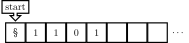
\includegraphics{res/turing_add1_1}
        \caption{$δ(\sstart, \sta) = (s_\text{overflow}, \sta, 1)$}
    \end{subfigure}
    
    \begin{subfigure}{.5\textwidth}
        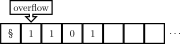
\includegraphics{res/turing_add1_2}
        \caption{$δ(s_\text{overflow}, \one) = (s_\text{overflow}, \one, 1)$}
    \end{subfigure}
    
    \begin{subfigure}{.5\textwidth}
        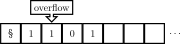
\includegraphics{res/turing_add1_3}
        \caption{$δ(s_\text{overflow}, \one) = (s_\text{overflow}, \one, 1)$}
    \end{subfigure}
    
    \begin{subfigure}{.5\textwidth}
        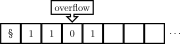
\includegraphics{res/turing_add1_4}
        \caption{$δ(s_\text{overflow}, \zer) = (s_\text{return}, \one, -1)$}
    \end{subfigure}
    
    \begin{subfigure}{.5\textwidth}
        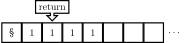
\includegraphics{res/turing_add1_5}
        \caption{$δ(s_\text{return}, \one) = (s_\text{return}, \one, -1)$}
    \end{subfigure}
    
    \begin{subfigure}{.5\textwidth}
        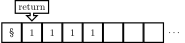
\includegraphics{res/turing_add1_6}
        \caption{$δ(s_\text{return}, \one) = (s_\text{return}, \one, -1)$}
    \end{subfigure}
    
    \begin{subfigure}{.5\textwidth}
        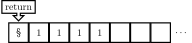
\includegraphics{res/turing_add1_7}
        \caption{$δ(s_\text{return}, \sta) = (s_\text{halt}, \sta, 0)$}
    \end{subfigure}
    
    \begin{subfigure}{.5\textwidth}
        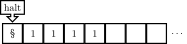
\includegraphics{res/turing_add1_8}
        \caption{$δ(s_\text{halt}, \sta) = (s_\text{halt}, \sta, 0)$}
    \end{subfigure}
    
    \caption{The complete run of $\mathbb A_\text{add1}$ on $\one\one\zer\one$}
    \label{fig:complete run}
\end{figure*}

\begin{defin}
    Let $\mathbb A$ be a Turing machine.
    
    \begin{enumerate}
        \item
          $\mathbb A$ \emph{computes} the partial function that maps each
          $x$ with a complete run to $\mathbb A(x)$ and is undefined for all
          other strings.
        \item
          $\mathbb A$ \emph{accepts} all $x$ such that
          $\mathbb A(x) = \one$ and \emph{rejects} them if
          $\mathbb A(x) = \zer$.
        \item
          A partial function on $\lbrace \sta, \emp, \zer, \one \rbrace^*$ is
          \emph{computable} if there is a Turing machine computing it.
        \item
          A subset of $\lbrace \sta, \emp, \zer, \one \rbrace^*$, i.e.~a
          problem, is \emph{decidable} if there is a Turing machine computing
          its characteristic function.
        \item
          A problem is called \emph{semi-decidable} or \emph{computably
          enumerable} if there is a Turing machine accepting precisely the
          elements of the problem.
    \end{enumerate}
\end{defin}

The last postulate of the definition above means that a problem is
semi-decidable if there is a Turing machine affirming membership of the
corresponding set but it might not be able to refute membership.

\begin{exam}
    We can encode a natural number $n$
    
    \begin{exlist}
    \item
      in tally notation
      \begin{align*}
        n & ↦ \underbrace{\one…\one}_{n\text{-times}}, \quad \text{if } n > 0 \\
        0 & ↦ λ
      \end{align*}
    \item
      by its binary representation
      \begin{align*}
          n = 2^k + \sum_{i = 0}^{k-1} b_i 2^i & ↦ b_0…b_{k-1}\one, \quad
              \text{if } n > 0\\
                                             0 & ↦ \zer,
      \end{align*}
      or
    \item
      by a shifted and truncated form of its binary representation
      \begin{align*}
        n = 1 + \sum_{i = 0}^k b_i 2^i & ↦ b_0…b_k, \quad \text{if } n > 0\\
                                     0 & ↦ λ
      \end{align*}
    \end{exlist}
    
    In either case the set obtained by encoding $ℕ$ is easily seen to be
    decidable. In the first case, check that the string contains only copies
    of the bit $\one$. Indeed, this can be achieved by the Turing machine
    
    \[\mathbb A_\text{tally} = ( \lbrace \sstart, \shalt, \scheck, s_\text{accept}, s_\text{reject}, s_\text{rejectMR}\rbrace, δ)\]
    
    whose transition function is displayed in \cref{lst:tally encoding}.
    
    \lstinputlisting[float,
                     caption=A Turing machine checking whether the input is tally-encoded,
                     label=lst:tally encoding]{./listings/tally.hs}
    
    
    In the second case it suffices to check that the string has length $1$
    or ends in a $\one$, and in the third case every string is accepted.
\end{exam}

\subsubsection{Halting problem}

One can extend the alphabet of Turing machines by encoding characters
i.e.~assigning bit sequences to them. Very common encodings are
\textsc{ASCII} and \textsc{UTF-8}\footnote{See the Appendix for an
  \textsc{ASCII} encoding table and details on \textsc{UTF-8}.}. Using
either one of these encodings the string `haskell' is encoded as

\begin{lstlisting}
h         a         s         k         e         l         l
0110 1000 0110 0001 0111 0011 0110 1011 0110 0101 0110 1100 0110 1100
\end{lstlisting}

In this way we can encode a Turing machine as the \textsc{UTF-8}--encoding of
their transition function $δ$ written as a string as above. Note that
the set of states can implicitly be deduced from the transition function
as the set of acceptable first arguments of $δ$.

One of the fundamental theorems of theoretical computer science is the
existence of a universal Turing machine.

\begin{thm}
    There exists a Turing machine $\mathbb U$ that computes upon receiving
    the tuple $(\ulcorner \mathbb A \urcorner, x)$ as input, the output of
    Turing machine $\mathbb A$ on $x$ i.e.
    \[ \mathbb U(\ulcorner \mathbb A \urcorner, x) = y \Leftrightarrow \mathbb A (x) = y\]
\end{thm}

A natural question is:

Given a machine $\mathbb A$ and a string $x$. Does $\mathbb A$
halt on $x$?

It is one of the most fundamental results of theoretical computer
science that the halting problem is unsolvable.

\begin{thm}
    The halting problem is undecidable.
\end{thm}
\begin{proof}
    Assume there exists a Turing machine $\mathbb B$ that decides the
    halting problem i.e.~for all Turing machines $\mathbb A$ and all
    strings $x$
    
    \[ \mathbb B(\mathbb A, x) =
    \begin{cases}
      \one  & \text{if } \mathbb A \text{ halts on } x\\
      \zer  & \text{if } \mathbb A \text{ does not halt on } x
    \end{cases}\]
    
    Now using $\mathbb B$ construct a Turing machine $\mathbb B'$ such
    that
    
    \[ \mathbb B'(\mathbb A) = \one \Leftrightarrow \mathbb A \text{ does not halt on } \ulcorner \mathbb A\urcorner \]
    
    Now if $\mathbb B'(\mathbb B, \ulcorner \mathbb B\urcorner) = \one$
    then by definition of $\mathbb B'$ we find that
    $\mathbb B does not halt on \ulcorner \mathbb B\urcorner$. But by
    definiton of $\mathbb B$ this means that
    $\mathbb B(\mathbb B, \ulcorner \mathbb B \urcorner) = \zer$
\end{proof}


\section{Binary Trees and Their Automorphism Group}
%\input{./Inhalt/BinaryTrees}

\section{Definition and Elementary Properties of the First Grigorchuk Group}
%\input{./Inhalt/FirstGrigorchukGroup}

\chapter{Burnside's Problems}
%\input{./Inhalt/HistoryOfBurnsidesProblems}

\section{A Counterexample to the Unbounded Burnside Problem}
%\input{./Inhalt/BurnsidesProblem}

\section{Growth of the First Grigorchuk Group}
%\input{./Inhalt/Growth}

\clearpage
\appendix
\chapter{Appendix}\label{sec:Appendix}
%\input{./Inhalt/Appendix}

\backmatter
\vspace{\fill}
\printbibliography

\listoftodos
\end{document}
